\documentclass[12pt]{article}
\usepackage[utf8]{inputenc}
\usepackage{amsmath, amssymb, amsthm, graphicx, fancyvrb, enumitem, titlesec, setspace, float, fancyvrb, minted}
\usepackage[dvipsnames]{xcolor}
\usepackage[top=1in, bottom=1in, left=1.25in, right=1.25in]{geometry}
\titleformat{\section}{\normalfont\bfseries}{}{0em}{}
\titlespacing*{\section}{0pt}{1.5ex plus .2ex minus .2ex}{0.8ex plus .1ex}


\begin{document}
\noindent Andre Winkel \hfill \today \\
\rule{\textwidth}{0.4pt} \vspace{0em}
\begin{center} \large{Lab 7} \end{center} \vspace*{0em}

\section*{Problem 1: Aliasing of sinusoids}
In this problem, we consider the sinusoid
\begin{equation} \notag
    x(t)=\cos(10\pi t).
\end{equation}
In order to plot the waveform of $x(t)$ for $0\le t < 5$ using MATLAB, we consider the sampled version
\begin{equation} \notag
    x[n]=x(nT_s)=\cos(10T_s\pi n)
\end{equation}

\begin{enumerate}[label=\textbf{\alph*)}, leftmargin=2.6em]
\item For $T_s=0.001$ sec, we observe
\begin{figure} [H]
    \centering
    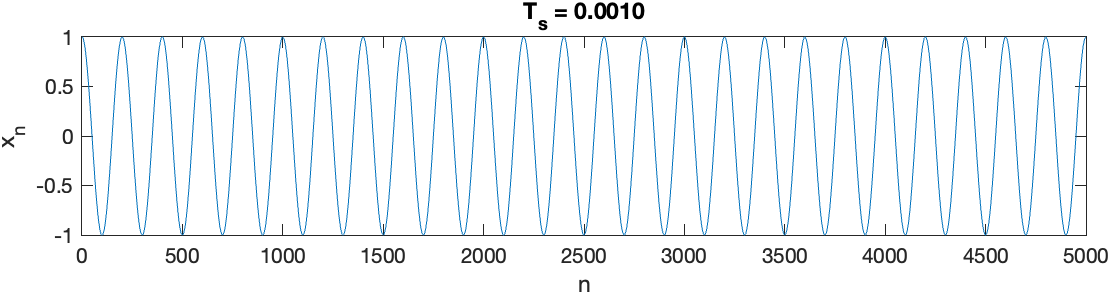
\includegraphics[width=0.8\linewidth]{1a.png}
\end{figure}
\item For $T_s=0.01$ sec, we observe
\begin{figure} [H]
    \centering
    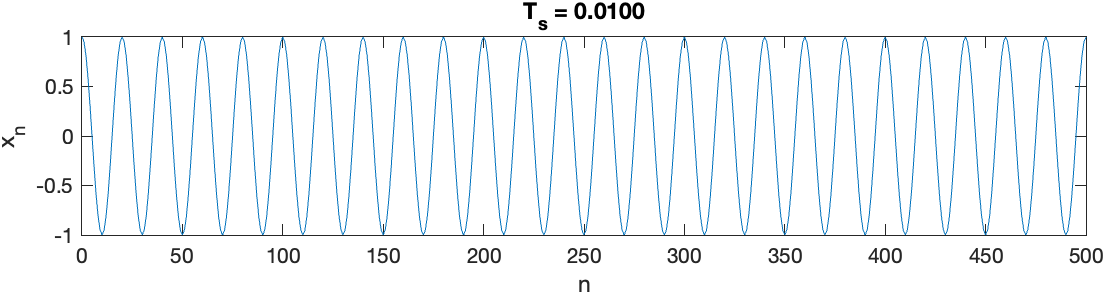
\includegraphics[width=0.8\linewidth]{1b.png}
\end{figure}
\item For $T_s=0.1$ sec, we observe
\begin{figure} [H]
    \centering
    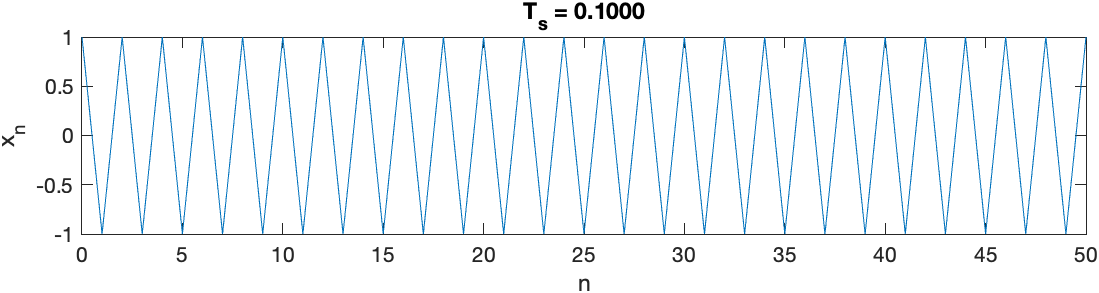
\includegraphics[width=0.8\linewidth]{1c.png}
\end{figure}
\item For $T_s=0.1923$ sec, we observe
\begin{figure} [H]
    \centering
    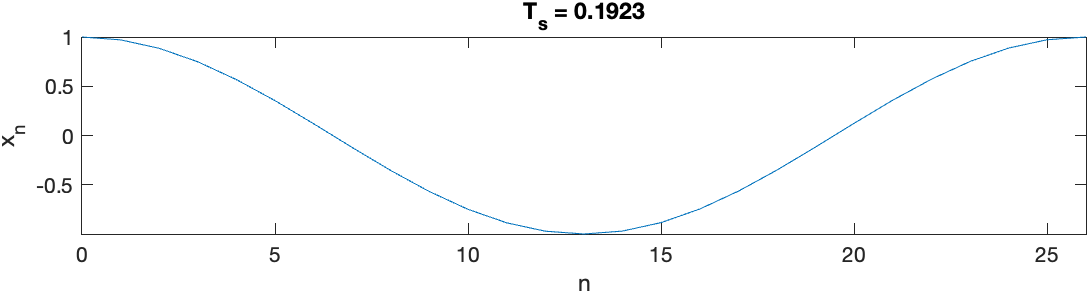
\includegraphics[width=0.8\linewidth]{1d.png}
\end{figure}
\item For $T_s=0.2$ sec, we observe
\begin{figure} [H]
    \centering
    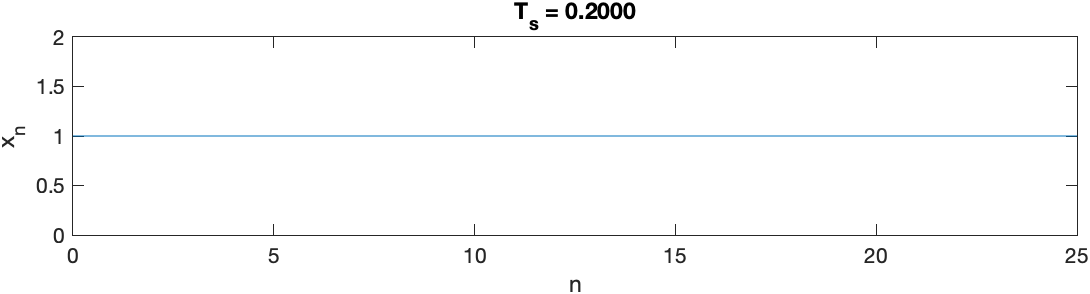
\includegraphics[width=0.8\linewidth]{1e.png}
\end{figure}

\begin{minted}[frame=single, fontsize=\small, linenos, bgcolor=white]{matlab}
T_s = [0.001, 0.01, 0.1, 0.1923, 0.2]

for i=1:length(T_s)
    T=T_s(i)
    n = 0:5/T
    x_n = cos(10*T*pi*n)

    subplot(length(T_s), 2, i)
    plot(n, x_n)
    xlabel('n')
    ylabel('x_n')
    axis tight
    title(sprintf('T_s = %.4f', T));
end
\end{minted}
\end{enumerate}
In this problem, we note that for both \textbf{d)} and \textbf{e)}, we are unable to observe 25 cycles. This is primarily because we are under-sampling the signal at those values for $T_s$. As we have what is effectively a 5 Hz signal, as we approach sampling rates that are closer to this frequency we will be able to observe less of the signal, therefore exhibiting aliasing. For example, if we sample a periodic signal on its period, we will always observe the same value, which is what we see in \textbf{e)}.

\section*{Problem 2: Aliasing of chirps}
In this problem, we consider the chirp
\begin{equation} \notag
    x(t)=\cos\left(\frac{\pi t^2}{64}\right),
\end{equation}
and analyze this signal for $0\le t<128$ by observing its sampled version given by
\begin{equation} \notag
    x[n]=\cos\left(\frac{\pi T^2_sn^2}{64}\right).
\end{equation}
\begin{enumerate}[label=\textbf{\alph*)}, leftmargin=2.6em]

\item Observing the chirp signal and considering its linearly increasing frequency, we can determine the signal is aperiodic. This is because of the previously mentioned property of chirp signals, their linearly increasing frequency. This indicates the signal does not inherently repeat itself, thus being aperiodic.

\item Below, we can observe our very rough sketch of $x(t)$. We can see that on average, the crests become closer together as time proceeds, which implies the frequency increases linearly with time. Changing the tolerance for our approximation also allows slightly better observation as time increases.
\begin{figure} [H]
    \centering
    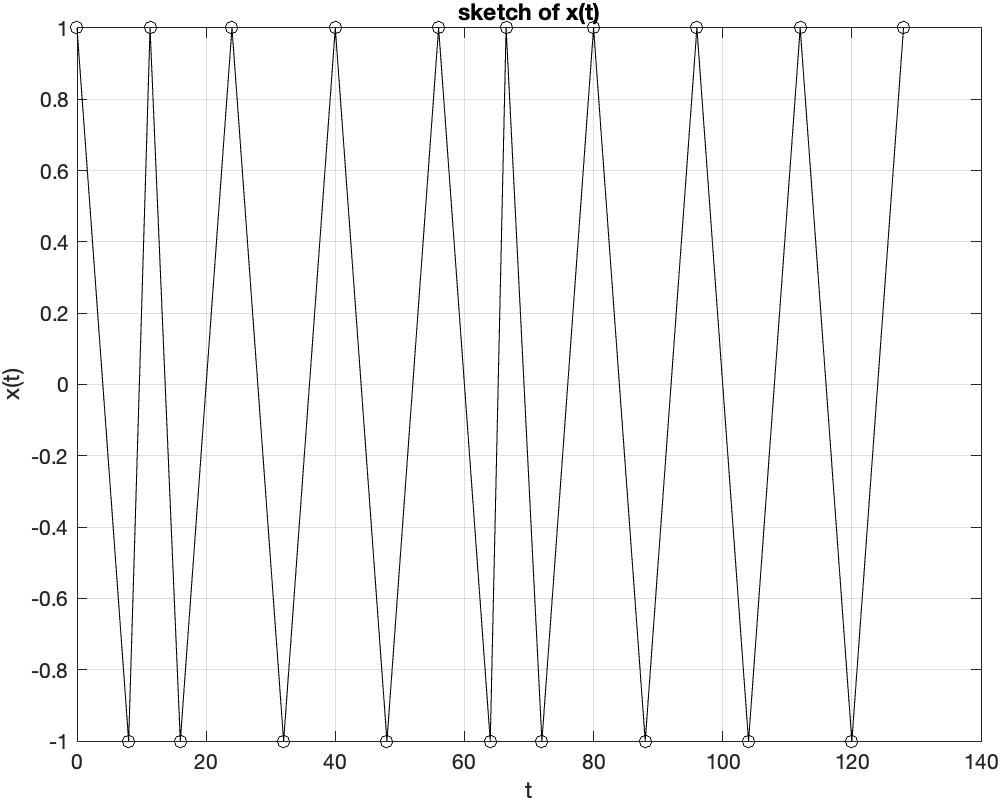
\includegraphics[width=0.5\linewidth]{2b.png}
\end{figure}
\begin{minted}[frame=single, fontsize=\small, linenos, bgcolor=white]{matlab}
clear

% sketch of x_t
t = 0:1/64:128;
x_t = cos(pi*t.^2/64);
tol = 1e-5;

a_k = t(abs(x_t - 1) < tol);
b_k = t(abs(x_t + 1) < tol);

t_plot = sort([a_k b_k]);
t_plot(2:11) = [];

n = 0:length(t_plot)-1;
x_plot = (-1).^(n);

plot(t_plot, x_plot, 'k-o');
xlabel('t');
ylabel('x(t)');
title('sketch of x(t)');
grid on;
\end{minted}

\item Setting $T_s=1$ and plotting $x[n]$ for $0\le n<\frac{128}{T_s}$, we can observe the following plot:
\begin{figure} [H]
    \centering
    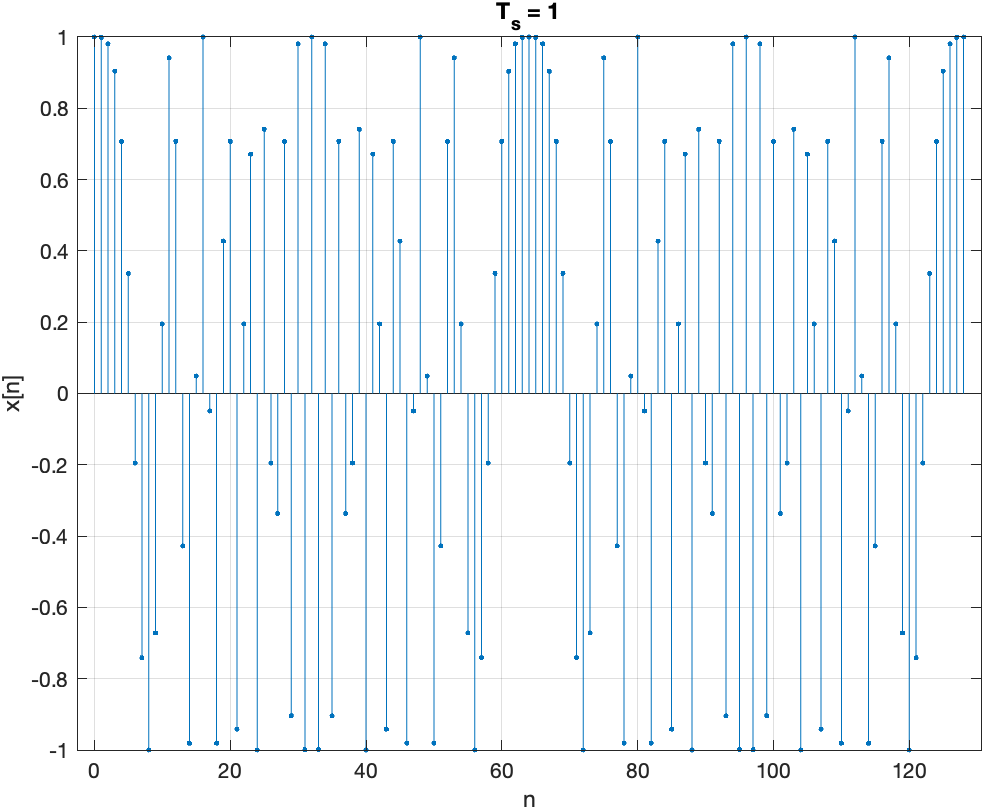
\includegraphics[width=0.5\linewidth]{2c.png}
\end{figure}
We can observe periodicity in the sampled signal, which is a discrepancy between $x[n]$ and $x(t)$ in terms of behavior. This is primarily due to aliasing as our sampling rate is not only too slow, but is occasionally in phase with the original signal as it increases in frequency.

\begin{minted}[frame=single, fontsize=\small, linenos, bgcolor=white]{matlab}
clear

T_s = 1;
n = 0:128;
x_n = cos(pi * T_s^2 * n.^2 / 64);

stem(n, x_n, '.', 'filled');
xlabel('n');
ylabel('x[n]');
title('T_s = 1');
grid on;
\end{minted}

\item Setting $T_s=0.1$ and plotting $x[n]$ for $0\le n<\frac{128}{T_s}$, we can observe the following plot:
\begin{figure} [H]
    \centering
    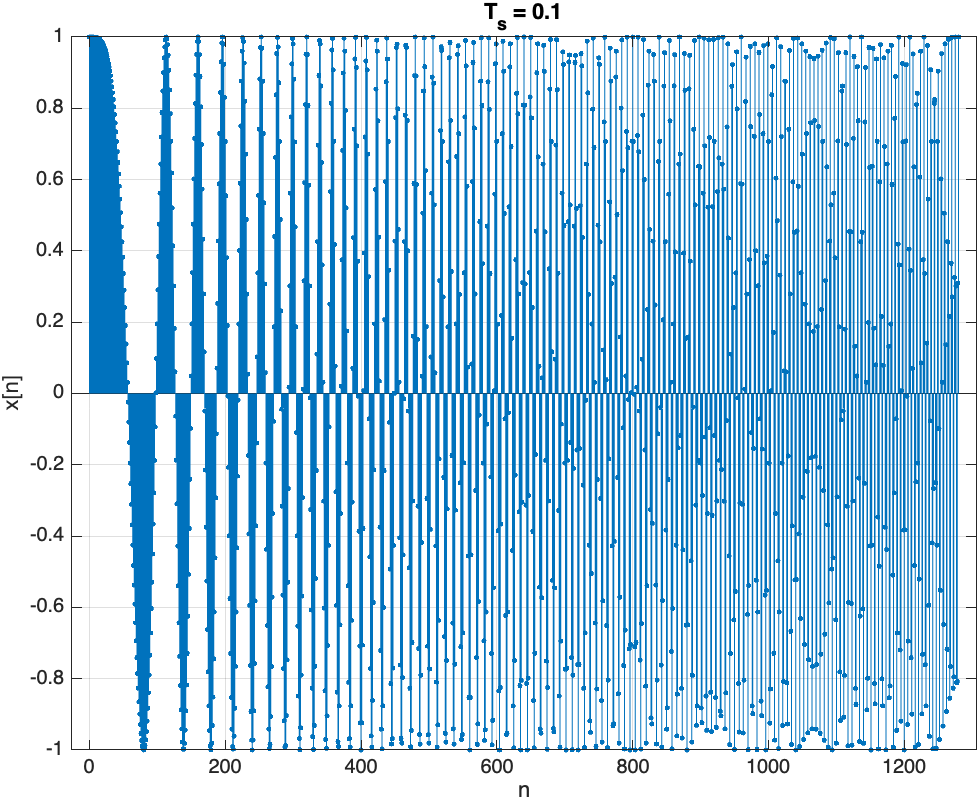
\includegraphics[width=0.5\linewidth]{2d.png}
\end{figure}
Here, we see a fairly similar signal to the signal that was sketched in part \textbf{b)}, in slightly higher resolution (yet less accurate). This is not necessarily a universal solution for this signal as it only works for the range of frequencies we are viewing. If we plot $x[n]$ for $0\le n<\frac{1024}{T_s}$, we observe the following plot:
\begin{figure} [H]
    \centering
    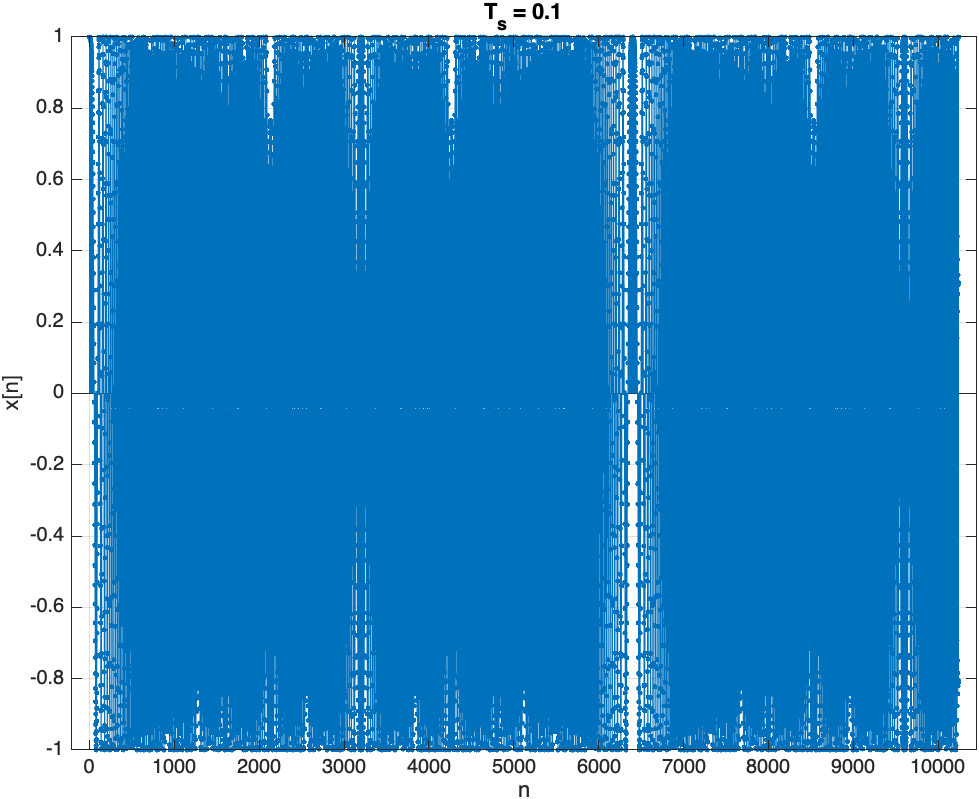
\includegraphics[width=0.5\linewidth]{2e.png}
\end{figure}
Here, we can better observe the apparent periodicity in our sampled signal as a result of aliasing, especially as the signal appears to repeat itself at around $t=6400$.

\begin{minted}[frame=single, fontsize=\small, linenos, bgcolor=white]{matlab}
clear

T_s = 0.1;
n = 0:1024/T_s;
x_n = cos(pi * T_s^2 * n.^2 / 64);

stem(n, x_n, '.', 'filled');
xlabel('n');
ylabel('x[n]');
title('T_s = 0.1');
grid on;
\end{minted}

\item We can conclude that using any value for our sampling rate, $T_s$, will never work for all possible intervals of $t$ due to aliasing. As our chirp signal linearly increases in frequency with respect to time, there will always be points for which the sampling rate results in aliasing, which is when our sampling rate is around the same frequency as our sampled signal. However, if we are attempting to observe a specific range of the signal, choosing any $T_s$ that works for this range, as shown in the first plot of part \textbf{(d)}, should be satisfactory. \\In conclusion, as our function sweeps through all frequencies, there is no possible value of $T_s$ that avoids aliasing, as the corresponding frequency will always be included in the chirp and will result in apparent periodicity.

\end{enumerate}

\end{document}